% !TeX root = ../dokumentation.tex

\chapter{Teamorganisation} \label{team_orga}

\section{Rollenverteilung}
    Zusätzlich zu den klassischen Scrum-Rollen Product-Owner, Scrum-Master und Entwickler 
    wurden im Projekt weitere Rollen eingeführt: Architekten und Service-Leads (vgl. \ref*{fig:Rollenverteilung}). 
    Grundsätzliches Ziel war es die Komplexität des Projektes durch Arbeitsteilung und feste Ansprechpartner abzufangen.
    Damit sollte auch eine Zusammenarbeit trotz verschiedener Kenntnisstände zu ermöglichen und einen Wissensaustausch zu erleichtern.   

    Die Aufgabe des Produkt-Owners ist es, den Wert des Produkts bzw. des Projekts
    zu maximieren. Mithilfe des Backlogs und der Priorisierung der Aufgaben darin stellt der Produkt Owner
    sicher, dass das Team an den richtigen Aufgaben arbeitet.
    Zusätzlich wurden in unserem Team die Storys vom Product Owner erstellt und die Estimation- sowie Planning-Meetings geplant.

    Ein Scrum-Master ist vergleichbar mit einem Teamleiter. Er kümmert sich darum, dass
    das Team (Entwickler und PO) ihrer Arbeit bestmöglich nachgehen können und schützt
    das Team vor ungewolltem Einfluss von außen. Zusammenfassend kann
    man sagen, dass der Scrum-Master dafür verantwortlich ist, dass sich das Team selbst
    organisieren und arbeiten kann. Der Scrum-Master hat auch die Aufgabe, darauf zu achten, dass das Team sich an die
    Scrum-Regeln hält, also alle Meetings regelmäßig durchgeführt werden und tritt, wenn nötig in den Meetings als Moderator auf.

    Die Architekten sind für die grundsätzliche Infrastruktur im Projekt zuständig. 
    Dazu entwarfen sie eine Service-übergreifende Architektur und bestimmten nach Evaluierung die eingesetzten Technologien.
    Ziel war es, dass die Architekten einen Gesamtüberblick über das Projekt behalten, 
    und somit Kommunikation zwischen den Services ermöglichen.
     
    
    Service-Leads sind die Ansprechpartner für die einzelnen Services. Dabei sollen sie einen detaillierteren Überblick über die Services behalten 
    und bei Fragen des Teams zur Verfügung stehen. 
    Da die Service-Leads einen besseren Überblick über den Service haben, 
    übernehmen Sie standardmäßig die Reviews von service-spezifischen Tickets und Pull-Requests in den Service-Repositories.

    \begin{figure}[!hbt]
        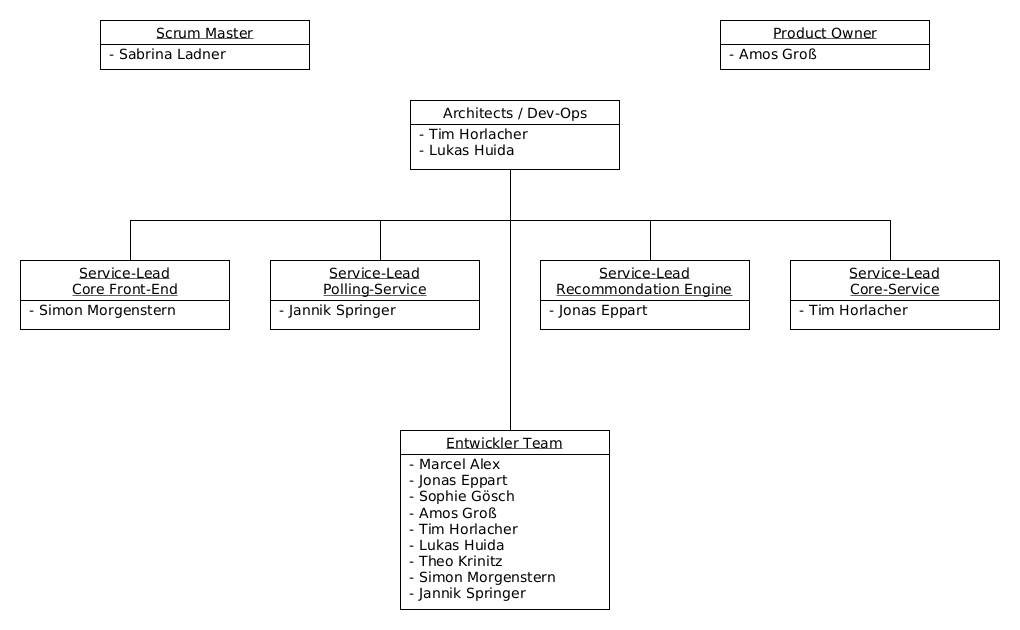
\includegraphics[width=\linewidth]{ProjectOrganigramm2.png}
        \caption{Rollenverteilung}
        \label{fig:Rollenverteilung}
    \end{figure}
    
\section{Eingesetzte Technologien}
Im Folgenden wird erklärt, welche Technologien wir in diesem Projekt eingesetzt haben und weshalb diese gewählt wurden.

\subsection{Typescript} \label{sub:Typescript}
    Typescript ist ein Superset von JavaScript. Dabei wurden in dieser Sprache Programmierkonstrukte wie Klassen und Vererbungen sowie Typisierungen implementiert. Das hilft uns, besseren Code zu entwickeln als in JavaScript.
    Der Grund weshalb wir Typescript in diesem Projekt verwenden, lässt sich damit Begründen, dass in vorherigen Semestern diese Sprache schon des Öfteren in Projekten verwendet wurde und deshalb bei jedem Entwickler gewisse Grundkenntnisse
    gegeben sind. Daher kann Zeit eingespart werden, um eine neue Sprache zu lernen. Typescript wird in diesem Projekt bei jedem Service verwendet, dass heißt sowohl Backend Services als auch das Frontend werden in Typescript geschrieben.
\subsection{Node.js}
    Node.js ist eine Javascript Laufzeitumgebung, welches ermöglicht Javascript Code, ohne einen Browser auszuführen. Dies kann zum Beispiel für Backend Services verwendet werden. Dabei muss nicht zwingend Javascript verwendet werden,
    in unserem Projekt benutzen wir es in Verbindung mit Typescript. Dies hat denselben Grund, wie der aus Abschnitt \ref{sub:Typescript}.
\subsection{Express}
    Express ist ein Web-Framework welches im Zusammenhang mit Node.js benutzt wird. Diese Technologie kommt im \textit{Core-Service} zum Einsatz. Es erleichtert es einem in Typescript Web-Services zu entwickeln.
    Dazu wurde auf Express noch Apollo-Server verwendet, welches für den GraphQL Endpoint zuständig ist.
\subsection{Devcontainers}
    Ein Devcontainer erlaubt den Entwicklern das einfache Erstellen einer Entwicklungsumgebung auf ihrem lokalen System.
    Dabei werden alle benötigten Entwicklungstools innerhalb eines Containers installiert, in dem dann entwickelt werden kann.
    Durch Devcontainer können wir sicherstellen, dass Entwickler alle Tools, die sie zum Entwickeln brauchen, auf ihrem System benutzen können, ohne alles einzeln installieren zu müssen.
\subsection{Keycloak}
    Keycloak ist ein Identity and Access Management System. Es dient dazu die Account-Authentifizierung zu vereinfachen und übernimmt den größten Teil davon.
    So können einfach Account innerhalb mehreren Anwendungen benutzt werden. Keycloak wurde in diesem Projekt verwendet, um die Authentifizierung bei den einzelnen Services zu vereinfachen.
\subsection{GraphQL}
    GraphQL ist eine Datenabfrage- und Manipulationssprache. Ein Client kann durch GraphQL die genaue Struktur der benötigten Daten selbst definieren.
    Eine REST-API gegenüber liefert nur eine konkrete Datenstruktur.
    In diesem Projekt haben wir uns für GraphQL entschieden, um gezielter Daten abzufragen und somit den Datenverkehr zwischen Client und Server möglichst minimal zu halten.
\subsection{TypeORM}
    TypeORM ist ein \ac{ORM} für das Javascript. Es erleichtert das Nutzen einer Datenbank, da man sich nicht mit \ac{SQL} Befehlen beschäftigen muss, sondern sich nur Gedanken um die Struktur seiner Daten machen muss.
    Auf der Datenstruktur baut TypeORM dann die Datenbank mit allen Tabellen. Das praktische ist, man kann TypeORM in Klassen mit Annotations benutzen, heißt man eine Klasse schreiben, die dann für die Datenbank benutzt wird
    aber auch gleichzeitig für den Programmcode. Um unsere Klassen auch für GraphQL zu verwenden, nutzen wir zusätzlich TypeGraphQL, welches Klassen automatisch in GraphQL Objekte konvertiert.
\subsection{PostgreSQL}
    PostgreSQL ist ein relationales Datenbankmanagement-System. Es wird in diesem Projekt verwendet, um die Datenbank zu verwalten. In dieser Datenbank werden alle notwendigen Daten erfasst.
    Die Entscheidung auf PostgreSQL wurde getroffen, da dieses Produkt Open-Source und kostenlos ist.    
\subsection{Git}
    Git ist ein Versionsverwaltungssystem. Es wird in diesem Projekt verwendet, um unseren Code zu verwalten. Als Plattform für Git nutzen wird \textit{Github}.
    Dazu dient es das unsere Pipelines ausgeführt werden können, da diese mit Github Verbunden sind.
\subsection{K3S}
    K3S ist im Endeffekt ein Kubernetes in leichtgewichtig. Damit ist es wesentlich einfacher ein Kubernetes Cluster aufzusetzen als mit dem richtigen Kubernetes auch \textit{k8s} genannt.
    K3S hat hierbei keine wirklichen Nachteile für unser Projekt, als wenn wir \textit{k8s} benutzen würden. Kubernetes für uns den Vorteil das es eine Containerorchestrierung-Plattform ist.
    Zum Beispiel ist es dann möglich Services als Cronjob auszuführen, was wir für den Polling-Service benutzen. Alternativ hätte man auch das ganze System nur in Docker aufsetzten können, hätte dann aber 
    nicht Flexibilität wie wir sie jetzt haben, da Container Orchestriert verwenden.
\subsection{Traefik}
    Traefik ist ein Reverse-Proxy, welcher sich auch um die Verwaltung von \ac{SSL} Zertifikaten kümmert. Er wird dafür verwendet um mehrere Anwendungen auf dem Projekt Server zu hosten.
    Zum Beispiel wird \textit{skiosa.de} und \textit{argocd.dev.skiosa.de} auf dem gleichen Server gehosted und Traefik verwalten den Netzwerkverkehr so, dass die korrekte Anfrage an den richtigen Service geht.
    Als alternative hätte man ein \textit{Nginx} benutzen können, hier wäre aber der Konfigurationsaufwand größer.
\subsection{Argo CD}
    ArgoCD ist eine deklarative \ac{CD} Software. Diese verwaltet alle unseren Kubernetes Konfigurationen, dabei kann es auch automatisch neue Builds unseres Projektes deployen.
    ArgoCD dient nur als Erleichterung für die Entwickler, man könnte alle Kubernetes Konfigurationen auch mit Skripten automatisiert verwalten lassen. Jedoch bietet ArgoCD eine übersichtliche UI,
    welche es auch Entwicklern, die kein Verständnis von Kubernetes haben, ermöglicht ihre Software in der Produktion zu beobachten.
\subsection{Drone}
    \textit{Drone.io} ist ein \ac{CI} Tool. Dies ermöglicht es uns \ac{CI/CD} Pipelines zu bauen. Was dem Projekt bzw. den Entwicklern hilft professionell Code zu entwickeln, da Tests und Builds automatisch erfolgen.
    Dazu ist immer den Stand des Master-Branches direkt deployed und kann auch von Benutzer getestet werden, um schneller Fehler zu finden. Als alternative hätte man auch Github Actions benutzen können, was einen geringeren
    Aufwand in der Ersteinrichtung hätte, jedoch wären wir dort bei Privaten Repositories limitiert was Ressourcen betrifft. Ein Vorteil von \textit{Drone.io} ist, dass es selber gehosted wird und somit eine bessere Privacy gewährt.
\subsection{SonarQube}
    SonarQube ist eine Software, welche Code analysieren kann und dabei auch zum Beispiel Sicherheitslücken erkennt.
    Es wird in diesem Projekt verwendet, um den Code zu analysieren, um dadurch wiederum die Qualität zu verbessern.
    Dabei wird bei jedem Pull-Request der Code überprüft und ein Entwickler erkennt direkt, ob zum Beispiel Bugs gefunden wurden oder sogenannte \textit{Code-Smells}. 
    Diese können zum Beispiel aufkommen, wenn vergessen wurde, nicht genutzte \textit{Imports} zu entfernen.
    Des Weiteren wird auch überprüft ob duplizierter Code vorhanden ist.

\section{Eingesetzte Collaboration Technologien} 
\subsection{Jira}
    Jira ist ein Issue-Tracking-System, das für die Projekt-Management- und Projekt-Management-Prozesse verwendet wird.
    In Jira können Tickets erstellt, zugeordnet und bearbeitet werden. Sie lassen sich einem Sprint zuordnen und im Kanban Board visualisieren.
    Zusätzlich lassen sich einfach Diagramme erstellen, die die Projekt-Management-Prozesse darstellen.
    In unserem Projekt haben wir uns für Jira entschieden, da die meisten es aus ihrer Praxisphase bereits kannten.
    Für unser Projekt wurde auch das Kanban Board verwendet, diese hatte mehrere Swimlanes, welche den Status eines Tickets präsentiert haben.
    Die Swimlanes beinhalteten folgenden Status:
    \begin{itemize}
        \item Open
        \item In Progress
        \item Needs Review
        \item In Review
        \item Done
    \end{itemize}
    Sobald von einem Ticket der Status verändert wurde, wird das Ticket auch in der Swimlane sich in die korrekte Spalte bewegen. Ebenso wenn man ein Ticket in eine andere Swimlane bewegt hat, hat sich der Status geändert.
    Der Status wurde Beispielsweise benutzt, um besseres Filtern zu ermöglichen, oder direkt zu erkennen welches Tickets fertig sind, da diese dann durchgestrichen waren.
    \begin{figure}[!hbt]
        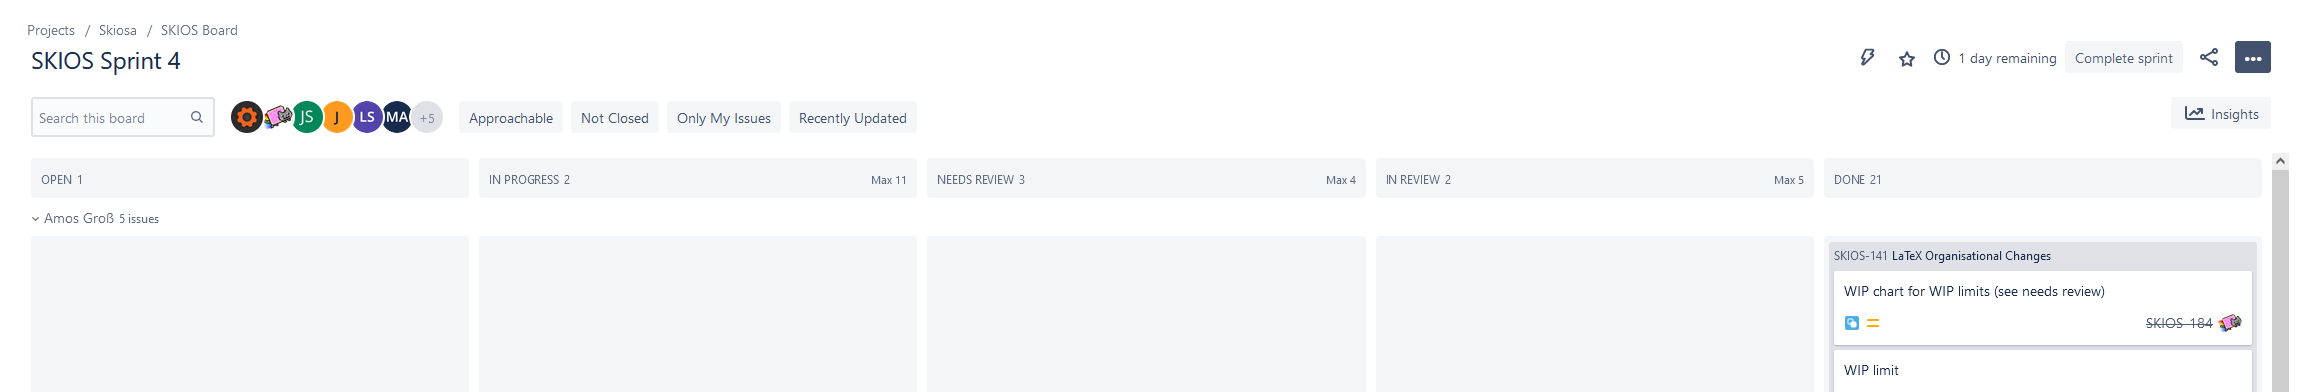
\includegraphics[width=\linewidth]{jiraSwimlanes.png}
        \caption{Jira-Swimlanes}
        \label{fig:Jira-Swimlanes}
    \end{figure}  
    Des Weiteren haben wir in den einzelnen Swimlanes \ac{WIP} genutzt, um einen Projekt-Fluss zu gewährleisten. Die \ac{WIP} sieht man in den Titel einer Swimlane, wie in \ref{fig:Jira-Swimlanes} zu sehen.
    Sobald ein \ac{WIP} Limit überschritten wurde, ist die ganze Swimlane rot hervorgehoben und jedes Team Mitglied erkennt sofort, dass ein Problem vorliegt bzw. dort Tickets abgearbeitet werden müssen.
\subsection{Github(Pull Requests)}
    Für jede Story wird ein eigener Pull-Request auf Github erstellt. Dieser wird von den Architekten und den Service-Leads überprüft, um anschließend in die
    produktive Anwendung integriert zu werden.  Pull Request wurden verwendet, um immer ein funktionierendes Inkrement des Produkts zu gewährleisten.
    Der Zustand der Pull-Request wird automatisch mit den Tickets in Jira synchronisiert. Das heißt, sobald ein neuer Branch mit dem Ticketnamen erstellt wird,
    geht das Ticket von \textit{Open} in den Status \textit{In Progress}. Anschließend wenn ein Pull-Request eröffnet wird welchen den Branch beinhaltet der dem Ticker zugeordnet ist,
    wird der Status von \textit{In Progress} in \textit{Needs Review} verändert. Hier muss dann ein Entwickler manuell das Ticket in \textit{In Review} verschieben da er seinen Namen unter dem Feld \textit{Reviewer}
    eintragen muss. Wenn ein Entwickler das Ticket bzw. den Pull-Request überprüft hat und in den Master Branch\textit{merged}, wird der Status von \textit{In Review} in \textit{Done} geändert.
\subsection{Confluence}
    Confluence dient als Wiki-Plattform für das Projekt. Es dient dazu, um wichtige Entscheidungen/Requirements zu dokumentieren und zu vermitteln.
\subsection{Figma}
    Figma ist eine Software für die Erstellung von Prototypen/Mockups im Bereich UI/UX. Durch die kollaborativen Funktionen können mehrere Personen einen Prototyp erstellen.
    Da es sich um eine Webanwendung handelt können Mockups schnell geöffnet werden und jeder mit Zugriff kann sich über den aktuellen Arbeitsstand Infomieren.
    Vor einer Feature-Implementierung in der Software wurde zuerst immer ein Mockup in Figma dafür erstellt.

\section{Meetings}
Zur Koordination des Teams wurden während des Projektes für Scrum übliche Meetings abgehalten und teilweise an unsere Rahmenbedingungen angepasst.

\subsection{Sprint Planning}
Zu Beginn jedes Sprints findet einmalig das \glqq Sprint Planning\grqq~statt. Dem Namen entsprechend wird in diesem Meeting ein genereller Plan 
für den Sprint erstellt, wofür zuerst vom Product Owner ein Ziel für den Sprint festgelegt wird. Danach werden Tickets aus dem Backlog 
ausgewählt, welche für das Ziel relevant sind und innerhalb des Sprints bearbeitet werden sollen. Dabei wird auch eingeschätzt, wie viel in einem 
Sprint realistisch schaffbar ist. Hierzu werden in \glqq Estimation-Meetings\grqq~die Tickets bezüglich des jeweiligen Arbeitsaufwandes eingeschätzt.
Das Resultat eines \glqq Sprint Plannings\grqq~ist das Sprint-Ziel und der Sprint Backlog.

\subsection{Roadmap-Meeting}
Um im Voraus Storys für das Sprint Planning zu erstellen und auszuplanen erfolgt das \enquote{Roadmap-Meeting}.
Hierbei wurden die Storys, welche vom PO erstellt wurden, mit dem Architekten abgesprochen.
Ziel ist es innerhalb dieses Meetings Storys auf ihre technische Umsetzbarkeit zu kontrollieren und möglicherweise in kleinere aufzuteilen.
Dieses Meeting fand meistens an den Montagen vor den jeweiligen Estimation Meetings statt.

\subsection{Estimation-Meeting}
Innerhalb des \glqq Estimation-Meetings\grqq~werden neue, meist vom Product Owner erstellte Tickets vorgestellt. Nachdem Fragen zum Ticket
geklärt wurden, wird der Arbeitsaufwand des Tickets in Story-Points geschätzt, wobei Fibonacci-Zahlen von 1 bis 21 verwendet werden. Zum Schätzen
gibt jedes Teammitglied eine Zahl an (oder enthält sich) und am Ende wird die Zahl mit den meisten Stimmen übernommen. 
Dieses Meeting findet im Anschluss eines Dailys oder BI-Weeklys statt, wenn seit dem Letzten neue Tickets hinzugefügt wurden.

\subsection{Daily und BI-Weekly}
In \glqq Dailys\grqq~wird von jedem Teammitglied der aktuelle Stand erläutert und Probleme, wie blockierende Tickets oder aufgetretene 
Unklarheiten angesprochen. Normalerweise wird dieses Meeting dem Namen entsprechend täglich abgehalten, ist jedoch in unserem Fall nur einmal 
wöchentlich im Rahmen der Vorlesung vorgesehen. Um einen häufigeren Austausch zu ermöglichen haben wir zusätzlich ein 
\glqq BI-Weekly\grqq~eingeführt, welches inhaltlich dem Daily gleicht und ebenso wöchentlich abgehalten wird.

\subsection{Review}
Zum Abschluss eines Sprints finden \glqq Review\grqq~und danach \glqq Retro\grqq~statt. Im Review wird besprochen, was im Sprint erreicht 
wurde und wie dies den allgemeinen Fortschritt des Projektes beeinflusst. Dabei wird auch besprochen, was als Nächstes zu Erreichen ist. 
Als Resultat dessen kann der Produkt Backlog beeinflusst werden und Ideen für das Planning des nächsten Sprints gesammelt werden. 

\subsection{Retro}
In der \glqq Sprint-Retrospektive\grqq~oder kurz \glqq Retro\grqq~wird die Zusammenarbeit im Team mithilfe verschiedener Retro-Spiele bewertet. 
Dabei wird besprochen, was gut lief und weitergeführt werden sollte, welche Probleme aufgetreten sind, was im weiteren Verlauf des Projektes 
vermieden werden sollte sowie potenzielle Neuerungen, die eingeführt werden sollten. Dies resultiert in sogenannten Action Items, welche das 
besprochene konkretisieren.

